%\VignetteEngine{knitr::knitr}
%\VignetteIndexEntry{Factor Loading using Adaptive Shrinkage using flashr}
%\VignettePackage{flashr}

% To compile this document
% library('knitr'); rm(list=ls()); knit('flashr/vignettes/flashr-vig.Rnw')
% library('knitr'); rm(list=ls()); knit2pdf('flashr/vignettes/flashr-vig.Rnw');
% openPDF('flashr-vig.pdf')
% !Rnw weave = knitr

\documentclass[12pt]{article}\usepackage[]{graphicx}\usepackage[usenames,dvipsnames]{color}
%% maxwidth is the original width if it is less than linewidth
%% otherwise use linewidth (to make sure the graphics do not exceed the margin)
\makeatletter
\def\maxwidth{ %
  \ifdim\Gin@nat@width>\linewidth
    \linewidth
  \else
    \Gin@nat@width
  \fi
}
\makeatother

\definecolor{fgcolor}{rgb}{0.345, 0.345, 0.345}
\newcommand{\hlnum}[1]{\textcolor[rgb]{0.686,0.059,0.569}{#1}}%
\newcommand{\hlstr}[1]{\textcolor[rgb]{0.192,0.494,0.8}{#1}}%
\newcommand{\hlcom}[1]{\textcolor[rgb]{0.678,0.584,0.686}{\textit{#1}}}%
\newcommand{\hlopt}[1]{\textcolor[rgb]{0,0,0}{#1}}%
\newcommand{\hlstd}[1]{\textcolor[rgb]{0.345,0.345,0.345}{#1}}%
\newcommand{\hlkwa}[1]{\textcolor[rgb]{0.161,0.373,0.58}{\textbf{#1}}}%
\newcommand{\hlkwb}[1]{\textcolor[rgb]{0.69,0.353,0.396}{#1}}%
\newcommand{\hlkwc}[1]{\textcolor[rgb]{0.333,0.667,0.333}{#1}}%
\newcommand{\hlkwd}[1]{\textcolor[rgb]{0.737,0.353,0.396}{\textbf{#1}}}%

\usepackage{framed}
\makeatletter
\newenvironment{kframe}{%
 \def\at@end@of@kframe{}%
 \ifinner\ifhmode%
  \def\at@end@of@kframe{\end{minipage}}%
  \begin{minipage}{\columnwidth}%
 \fi\fi%
 \def\FrameCommand##1{\hskip\@totalleftmargin \hskip-\fboxsep
 \colorbox{shadecolor}{##1}\hskip-\fboxsep
     % There is no \\@totalrightmargin, so:
     \hskip-\linewidth \hskip-\@totalleftmargin \hskip\columnwidth}%
 \MakeFramed {\advance\hsize-\width
   \@totalleftmargin\z@ \linewidth\hsize
   \@setminipage}}%
 {\par\unskip\endMakeFramed%
 \at@end@of@kframe}
\makeatother

\definecolor{shadecolor}{rgb}{.97, .97, .97}
\definecolor{messagecolor}{rgb}{0, 0, 0}
\definecolor{warningcolor}{rgb}{1, 0, 1}
\definecolor{errorcolor}{rgb}{1, 0, 0}
\newenvironment{knitrout}{}{} % an empty environment to be redefined in TeX

\usepackage{alltt}

\newcommand{\CountClust}{\textit{CountClust}}
\newcommand{\flashr}{\textit{flashr}}
\usepackage{dsfont}
\usepackage{cite}




\RequirePackage{/Library/Frameworks/R.framework/Versions/3.3/Resources/library/BiocStyle/resources/tex/Bioconductor}

\AtBeginDocument{\bibliographystyle{/Library/Frameworks/R.framework/Versions/3.3/Resources/library/BiocStyle/resources/tex/unsrturl}}


\author{Wei Wang, Kushal K Dey \& Matthew Stephens \\[1em] \small{\textit{Stephens Lab}, The University of Chicago} \mbox{ }\\ \small{\texttt{$^*$Correspondending Email: mstephens@uchicago.edu}}}

\bioctitle[Factor analysis with Adaptive Shrinkage using \flashr{}]{Factor analysis with Adaptive Shrinkage using \flashr{}}
\IfFileExists{upquote.sty}{\usepackage{upquote}}{}
\begin{document}

\maketitle

\begin{abstract}
  \vspace{1em}
  The \R{} package \flashr{} provides tools to perform factor analysis with adaptive shrinkage on the factor loadings and the factors and also provides means to visualization of the factor analysis results. The adaptive shrinkage is performed using the \textbf{ashr} package due to Stephens (2016).

  The package provides generic functions to visualize loadings data and post processing functions to analyze the factors estimated with focus on sparsity and the proportion of variance in the data explained by each factor. It also provides a list of features that play the key role in distinguishing the factors.

\vspace{1em}
\textbf{\flashr{} version:} 0.1.1 \footnote{This document used the vignette from \Bioconductor{} package \Biocpkg{DESeq2, CountClust} as \CRANpkg{knitr} template}

\end{abstract}




\newpage

\tableofcontents

\section{Introduction}

FLASH (Factor Loadings with Adaptive Shrinkage) is an extension of the adaptive shrinkage methods in \textbf{ashr} package due to Stephens (2016) to the domain of factor analysis. An important consideration in any factor analysis scheme are shrinkage and sparsity. There are many algorithms that perform Sparse Factor Analysis (check Engelhardt and Stephens), however determining the level of shrinkage is a challenging task for the user. FLASH solves this problem by adaptively selecting the level of shrinkage for factor loadings and factors.

\flashr{} offers 3 versions of FLASH (\textit{normal}, \textit{greedy} and \textit{backfitting}) to perform factor analysis with adaptive shrinkage. Also, it provides generic visualization tools to view and analyze the factor loadings along with post processing tools to check the proportion of variance explained and sparsity level of the different factors. Finally, it offers functions to select a list of features that drive the factors or play the most key role in distinguishing the features.

\section{\flashr{} Installation}

\flashr{} requires the packages \CRANpkg{ashr}, \CRANpkg{ggplot2}, \CRANpkg{irlba}, \CRANpkg{CountClust}, \CRANpkg{cowplot}, \CRANpkg{RColorBrewer}, \CRANpkg{grid}, \CRANpkg{gridExtra}. Also one needs the packages \CRANpkg{devtools}to install the developmental version of the \flashr{} which will be the most up-to-date version.

We install the Github version of the package.

\begin{knitrout}
\definecolor{shadecolor}{rgb}{0.969, 0.969, 0.969}\color{fgcolor}\begin{kframe}
\begin{alltt}
\hlstd{devtools}\hlopt{::}\hlkwd{install_github}\hlstd{(}\hlstr{"kkdey/flashr"}\hlstd{)}
\end{alltt}
\end{kframe}
\end{knitrout}

\begin{knitrout}
\definecolor{shadecolor}{rgb}{0.969, 0.969, 0.969}\color{fgcolor}\begin{kframe}
\begin{alltt}
\hlkwd{library}\hlstd{(flashr)}
\end{alltt}
\end{kframe}
\end{knitrout}

\section{Data preparation}

We install a single cell RNA-seq data across mouse embryo developmental stages due to Deng \textit{et al} 2014 \cite{Deng2014}. We load it as an ExpressionSet object.\begin{verb} singleCellRNASeqMouseDeng2014 \end{verb} data package due to Deng \textit{et al} is a processed version of the data publicly available at Gene Expression Omnibus (GEO:GSE45719: see \url{http://www.ncbi.nlm.nih.gov/geo/query/acc.cgi?acc=GSE45719}).

\begin{knitrout}
\definecolor{shadecolor}{rgb}{0.969, 0.969, 0.969}\color{fgcolor}\begin{kframe}
\begin{alltt}
\hlkwd{library}\hlstd{(devtools)}

\hlstd{read.data1} \hlkwb{=} \hlkwa{function}\hlstd{() \{}
  \hlstd{x} \hlkwb{=} \hlkwd{tempfile}\hlstd{()}
  \hlkwd{download.file}\hlstd{(}\hlstr{'https://cdn.rawgit.com/kkdey/singleCellRNASeqMouseDeng2014/master/data/Deng2014MouseEsc.rda'}\hlstd{,} \hlkwc{destfile}\hlstd{=x,} \hlkwc{quiet}\hlstd{=}\hlnum{TRUE}\hlstd{)}
  \hlstd{z} \hlkwb{=} \hlkwd{get}\hlstd{(}\hlkwd{load}\hlstd{((x)))}
  \hlkwd{return}\hlstd{(z)}
\hlstd{\}}

\hlstd{Deng2014MouseESC} \hlkwb{<-} \hlkwd{read.data1}\hlstd{()}

\hlcom{## Alternatively}
\hlcom{# install_github('kkdey/singleCellRNASeqMouseDeng2014')}
\end{alltt}
\end{kframe}
\end{knitrout}

We load the data

\begin{knitrout}
\definecolor{shadecolor}{rgb}{0.969, 0.969, 0.969}\color{fgcolor}\begin{kframe}
\begin{alltt}
\hlstd{deng.counts} \hlkwb{<-} \hlstd{Biobase}\hlopt{::}\hlkwd{exprs}\hlstd{(Deng2014MouseESC)}
\hlstd{deng.meta_data} \hlkwb{<-} \hlstd{Biobase}\hlopt{::}\hlkwd{pData}\hlstd{(Deng2014MouseESC)}
\hlstd{deng.gene_names} \hlkwb{<-} \hlkwd{rownames}\hlstd{(deng.counts)}

\hlstd{voom_out} \hlkwb{<-} \hlstd{limma}\hlopt{::}\hlkwd{voom}\hlstd{(deng.counts);}
\hlstd{voom_weights} \hlkwb{<-} \hlkwd{t}\hlstd{(voom_out}\hlopt{$}\hlstd{weights);}
\hlstd{voom_data} \hlkwb{<-} \hlkwd{t}\hlstd{(voom_out}\hlopt{$}\hlstd{E);}
\end{alltt}
\end{kframe}
\end{knitrout}


We apply FLASH on the data. We show here example of two versions of FLASH - the normal pooled FLASH on successive residuals and the greedy FLASH. We assume the number of factors to be $K=10$.

\begin{knitrout}
\definecolor{shadecolor}{rgb}{0.969, 0.969, 0.969}\color{fgcolor}\begin{kframe}
\begin{alltt}
\hlstd{ll} \hlkwb{<-} \hlkwd{flash.greedy}\hlstd{(voom_data,} \hlkwc{K}\hlstd{=}\hlnum{10}\hlstd{,} \hlkwc{flash_para} \hlstd{=} \hlkwd{list}\hlstd{(}\hlkwc{tol}\hlstd{=}\hlnum{1e-3}\hlstd{,} \hlkwc{maxiter_r1} \hlstd{=} \hlnum{50}\hlstd{,}
                \hlkwc{partype}\hlstd{=}\hlstr{"known"}\hlstd{,} \hlkwc{sigmae2_true} \hlstd{= voom_weights,}
                \hlkwc{nonnegative}\hlstd{=}\hlnum{FALSE}\hlstd{));}
\hlstd{ll} \hlkwb{<-} \hlkwd{flashpool}\hlstd{(voom_data,} \hlkwc{K}\hlstd{=}\hlnum{10}\hlstd{,} \hlkwc{tol}\hlstd{=}\hlnum{1e-3}\hlstd{,} \hlkwc{maxiter_r1} \hlstd{=} \hlnum{50}\hlstd{,}
                \hlkwc{partype}\hlstd{=}\hlstr{"known"}\hlstd{,} \hlkwc{sigmae2_true} \hlstd{= voom_weights);}
\end{alltt}
\end{kframe}
\end{knitrout}

We load the FLASH output from the greedy implementation of FLASH and then we process the output.

\begin{knitrout}
\definecolor{shadecolor}{rgb}{0.969, 0.969, 0.969}\color{fgcolor}\begin{kframe}
\begin{alltt}
\hlkwd{library}\hlstd{(flashr)}
\hlstd{ll_deng} \hlkwb{<-} \hlkwd{get}\hlstd{(}\hlkwd{data}\hlstd{(}\hlstr{"flash_deng_ex"}\hlstd{))}
\end{alltt}
\end{kframe}
\end{knitrout}

We postprocess the loadings and the factors from the FLASH output. We calculate the percentage of variance explained by each factor.

\begin{knitrout}
\definecolor{shadecolor}{rgb}{0.969, 0.969, 0.969}\color{fgcolor}\begin{kframe}
\begin{alltt}
\hlstd{postprocess_ll} \hlkwb{<-} \hlkwd{flash_factor_postprocess}\hlstd{(ll_deng}\hlopt{$}\hlstd{l,ll_deng}\hlopt{$}\hlstd{f, voom_data)}
\hlstd{pve_percentage} \hlkwb{<-} \hlkwd{c}\hlstd{(}\hlstr{""}\hlstd{,} \hlkwd{paste0}\hlstd{(}\hlstr{":PVE-"}\hlstd{,} \hlkwd{round}\hlstd{(postprocess_ll}\hlopt{$}\hlstd{PVE}\hlopt{*}\hlnum{100}\hlstd{,}\hlnum{0}\hlstd{),} \hlstr{"%"}\hlstd{))}
\end{alltt}
\end{kframe}
\end{knitrout}

We represent the loadings by a stacked barchart of the loadings obtained from the FLASH output. We keep aside the first factor as that represents the mean factor.

\begin{knitrout}
\definecolor{shadecolor}{rgb}{0.969, 0.969, 0.969}\color{fgcolor}\begin{kframe}
\begin{alltt}
\hlstd{omega} \hlkwb{<-} \hlstd{ll_deng}\hlopt{$}\hlstd{l}

\hlstd{annotation} \hlkwb{<-} \hlkwd{data.frame}\hlstd{(}
  \hlkwc{sample_id} \hlstd{=} \hlkwd{paste0}\hlstd{(}\hlstr{"X"}\hlstd{,} \hlkwd{c}\hlstd{(}\hlnum{1}\hlopt{:}\hlkwd{NROW}\hlstd{(omega))),}
  \hlkwc{label} \hlstd{=} \hlkwd{factor}\hlstd{(deng.meta_data}\hlopt{$}\hlstd{cell_type,}
                        \hlkwc{levels} \hlstd{=} \hlkwd{c}\hlstd{(}\hlstr{"zy"}\hlstd{,} \hlstr{"early2cell"}\hlstd{,}
\hlstr{"mid2cell"}\hlstd{,} \hlstr{"late2cell"}\hlstd{,}\hlstr{"4cell"}\hlstd{,} \hlstr{"8cell"}\hlstd{,} \hlstr{"16cell"}\hlstd{,}\hlstr{"earlyblast"}\hlstd{,}\hlstr{"midblast"}\hlstd{,}\hlstr{"lateblast"}\hlstd{) ) )}

\hlkwd{rownames}\hlstd{(omega)} \hlkwb{<-} \hlstd{annotation}\hlopt{$}\hlstd{sample_id}

\hlkwd{FactorGGStack}\hlstd{(}\hlkwc{loadings} \hlstd{= omega[,}\hlopt{-}\hlnum{1}\hlstd{],}
                \hlkwc{annotation} \hlstd{= annotation,}
                \hlkwc{palette} \hlstd{=} \hlkwd{c}\hlstd{(RColorBrewer}\hlopt{::}\hlkwd{brewer.pal}\hlstd{(}\hlnum{8}\hlstd{,} \hlstr{"Accent"}\hlstd{),RColorBrewer}\hlopt{::}\hlkwd{brewer.pal}\hlstd{(}\hlnum{4}\hlstd{,} \hlstr{"Spectral"}\hlstd{)),}
                \hlkwc{yaxis_label} \hlstd{=} \hlstr{"Development Phase"}\hlstd{,}
                \hlkwc{order_sample} \hlstd{=} \hlnum{TRUE}\hlstd{,}
                \hlkwc{figure_title} \hlstd{=} \hlstr{"Factor Loadings Structure Plot"}\hlstd{,}
                \hlkwc{legend_labels} \hlstd{= pve_percentage[}\hlopt{-}\hlnum{1}\hlstd{],}
                \hlkwc{scale}\hlstd{=}\hlnum{TRUE}\hlstd{,}
                \hlkwc{axis_tick} \hlstd{=} \hlkwd{list}\hlstd{(}\hlkwc{axis_ticks_length} \hlstd{=} \hlnum{.1}\hlstd{,}
                                 \hlkwc{axis_ticks_lwd_y} \hlstd{=} \hlnum{.1}\hlstd{,}
                                 \hlkwc{axis_ticks_lwd_x} \hlstd{=} \hlnum{.1}\hlstd{,}
                                 \hlkwc{axis_label_size} \hlstd{=} \hlnum{7}\hlstd{,}
                                 \hlkwc{axis_label_face} \hlstd{=} \hlstr{"bold"}\hlstd{))}
\end{alltt}
\end{kframe}
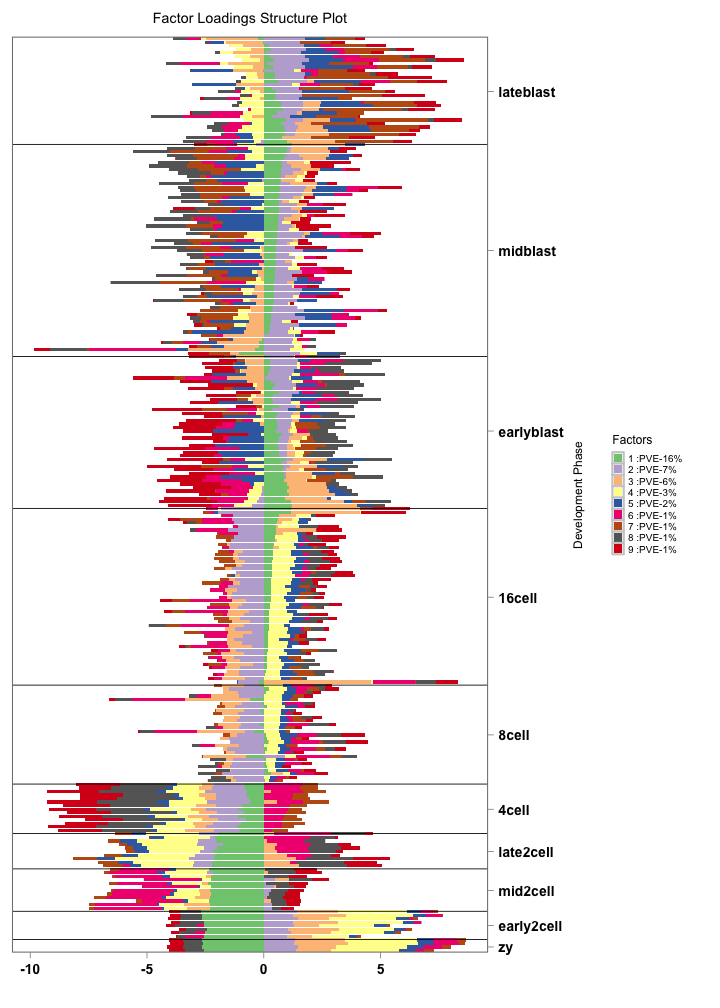
\includegraphics[width=5in,height=7in]{figure/flash_structure-1}

\end{knitrout}

We next look at a multi-grid bar chart representation of the factor loadings.

\begin{knitrout}
\definecolor{shadecolor}{rgb}{0.969, 0.969, 0.969}\color{fgcolor}\begin{kframe}
\begin{alltt}
\hlkwd{FactorGGBar}\hlstd{(}\hlkwc{loadings} \hlstd{= omega,}
            \hlkwc{annotation} \hlstd{= annotation,}
            \hlkwc{palette} \hlstd{=} \hlkwd{list}\hlstd{(}\hlstr{"mid"}\hlstd{=}\hlstr{"white"}\hlstd{,}
                           \hlstr{"low"}\hlstd{=}\hlstr{"red"}\hlstd{,}
                           \hlstr{"high"}\hlstd{=}\hlstr{"blue"}\hlstd{,}
                           \hlstr{"midpoint"}\hlstd{=}\hlnum{0}\hlstd{),}
            \hlkwc{yaxis_label} \hlstd{=} \hlstr{"Population Type"}\hlstd{,}
            \hlkwc{figure_title} \hlstd{=} \hlstr{" "}\hlstd{,}
            \hlkwc{axis_tick} \hlstd{=} \hlkwd{list}\hlstd{(}\hlkwc{axis_ticks_length} \hlstd{=} \hlnum{.1}\hlstd{,}
                             \hlkwc{axis_ticks_lwd_y} \hlstd{=} \hlnum{.1}\hlstd{,}
                             \hlkwc{axis_ticks_lwd_x} \hlstd{=} \hlnum{.1}\hlstd{,}
                             \hlkwc{axis_label_size} \hlstd{=} \hlnum{7}\hlstd{,}
                             \hlkwc{axis_label_face} \hlstd{=} \hlstr{"bold"}\hlstd{),}
            \hlkwc{legend_labels}\hlstd{=pve_percentage,}
            \hlkwc{scale}\hlstd{=}\hlnum{TRUE}\hlstd{,}
            \hlkwc{panel}\hlstd{=}\hlkwd{list}\hlstd{(}\hlkwc{panel_rows}\hlstd{=}\hlnum{2}\hlstd{,}
                       \hlkwc{panel_title}\hlstd{=}\hlstr{"Factor Loadings Bar plot"}\hlstd{,}
                       \hlkwc{panel_title_fontsize}\hlstd{=}\hlnum{10}\hlstd{,}
                       \hlkwc{panel_title_font}\hlstd{=}\hlnum{3}\hlstd{))}
\end{alltt}
\end{kframe}
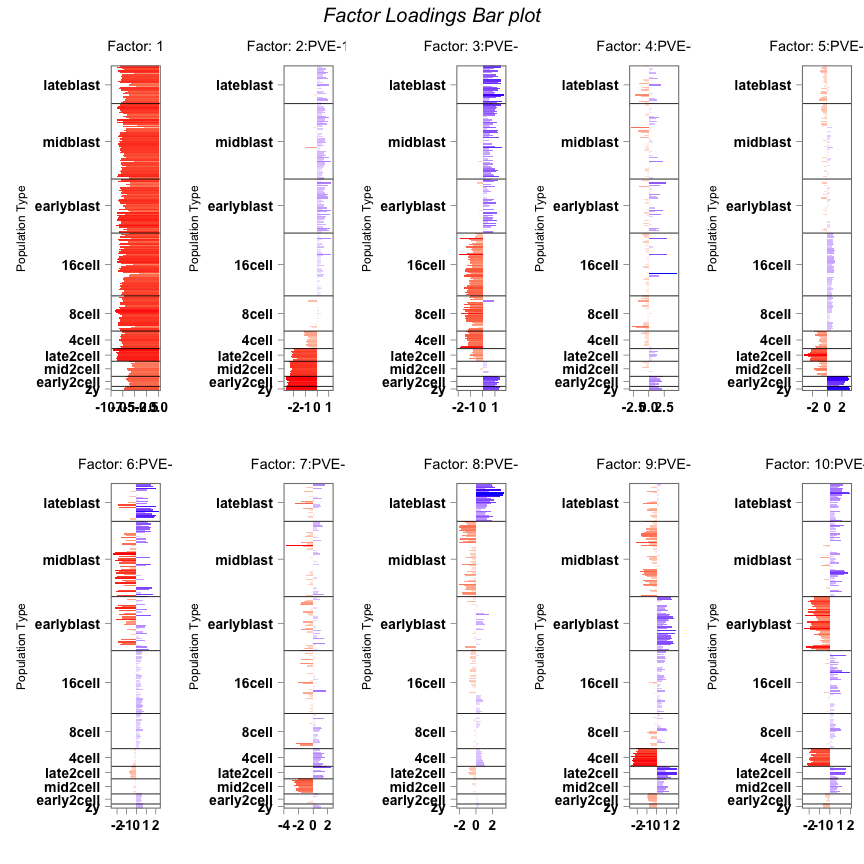
\includegraphics[width=6in,height=6in]{figure/flash_multipanel_grid-1}

\end{knitrout}






\end{document}
